\chapter{Billiard-AI}
In diesem Kapitel werden die gewählte Architektur wie auch die bisher erarbeiteten theoretischen Ansätze behandelt.
Weiterhin wird auf verschiedene Aspekte des Aufbaus und dessen Problematik eingegangen.

\section{Aufbau}
TODO: Beschreibung

\section{Architektur}
Die eigentliche Funktionalität wird in einer Core-Library untergebracht, welche nativ in C++ entwickelt wird. Das
Endprodukt soll aber weitaus mehr zu bieten haben, wie aus den Zielen ersichtlich wird. Deswegen wird in Unity eine
Interaktionsmöglichkeit geschaffen, worüber der Benutzer einerseits die Resultate visualisiert erhält und
andererseits der Core-Library seine nächsten Schritte mitteilen kann. Um dies zu erreichen, wird eine weitere native
Komponente erstellt, welche die Interaktion zwischen Unity und der Core-Library ermöglicht. Es ist dies eine C/C++-Bibliothek,
die ein C-Interface bereitstellt, welches in Unity geladen wird. Unity selbst erhält ebenfalls eine Abstraktionsschicht,
um die Nativen auf die Applikationsmodelle zu mappen. Eine Darstellung kann in Abbildung \ref{fig:top-level-architecture} entnommen
werden.

\begin{figure}[h!]
    \begin{center}
        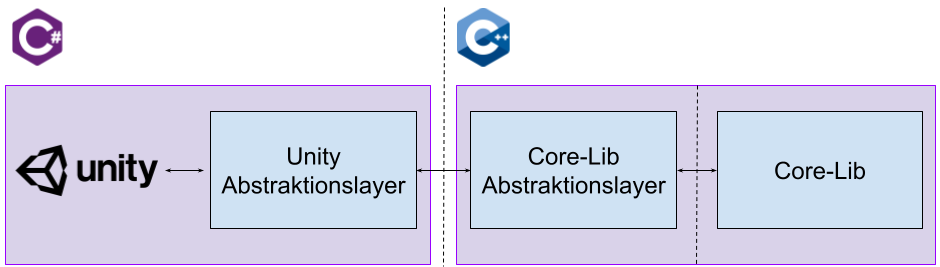
\includegraphics[width=0.8\linewidth]{../common/03_billiard_ai/resources/00_top_level_architecture.png}
    \end{center}
    \caption{Grobarchitektur - Applikationsumgebung}
    \label{fig:top-level-architecture}
\end{figure}

Die Core-Library selbst besteht aus mehreren Teilstücken. Es sind dies namentlich mitsamt Funktionalität die
folgenden:
\begin{description}
    \item[billiard\textunderscore capture] Erfasst den aktuellen Spielstand und stellt diesen im OpenCV-Format bereit.
    \item[billiard\textunderscore detection] Erstellt aus dem Spielstand eine interne Repräsentation, welchen den Status beschreibt.
    \item[billiard\textunderscore search] Verwendet den aktuellen Status wie auch eine zusätzliche Such-Beschreibung, um einen optimalen
    Stoss zu berechnen.
    \item[billiard\textunderscore physics] Stellt Funktionalität bereit, um physikalische Berechnungen durchzuführen.
\end{description}

\section{Die Suche - ein theoretisches Modell}